
\chapter{Détection des anomalies de la route}

Avec cette évolution dans le domaine des mobiles, il est possible de développer un système pratique et efficace à faible coût et
 recueilli divers types d'informations afin de détecter la qualité de la surface des routes et aussi les anomalies routières telles
  que les ralentisseurs et les nids de-poule.

\section{Related work}

\subsection{Wolverine}
Wolverine est \cite{bhoraskarWolverineTrafficRoad2012}une méthode non intrusive qui utilise  des données de capteurs des smartphones pour déterminer les conditions et l'état de la route, et utilise aussi des techniques d'apprentissage automatique “Machine learning” (clustering K-means et Support Vector Machine (SVM)) afin de la surveillance et suivi de l'état de la route
le chemin de ce travail consiste a deux étape: un algorithme pour réorienter virtuellement les axes de coordonnées d'un téléphone désorienté  et techniques d'apprentissage automatique pour identifier les événements de bosse et de freinage.\newline
Pour la 1ere étape ils ont développé une application qui traite les lectures de l'accéléromètre et du magnétomètre ainsi que les informations GPS et produit l'accélération linéaire du mobile, dans le cadre de référence du véhicule, ils ont développé un algorithme qui etude les axe x,y,z du téléphone et étude aussi les axes x’ y’ z’ de la véhicule.\newline
 La 2ème étape consistera à utiliser un algorithme d'apprentissage non supervisé de clustering K-means, avec K = 2, pour partitionner l'ensemble des points de données en deux classes; Ces classes sont ensuite étiquetées manuellement comme bosselées ou lisses (Bumby; smoothy)\newline
Une fois cet étiquetage manuel terminé, ils auront  un ensemble de points de données étiquetés. Ceux-ci sont ensuite utilisés pour former un classificateur Support Vector Machine. Ce SVM entraîné, à son tour, est utilisé pour classer les points de données qui sont générés pendant la phase de test, et donc pour prédire l'état du véhicule (Figure 2.1). \newline
\begin{figure}[h!]
  \center
  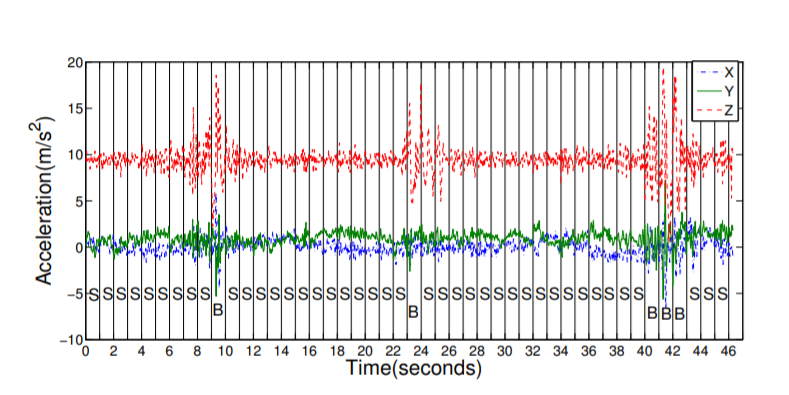
\includegraphics[width=0.75\textwidth]{Images/chapter2/relatedWork1.PNG}
 \caption{Accelerometer Data for three speedbreakers}
 \label{fig:graph}
  \end{figure}
  Et pour la détection du freinage du véhicule La technique utilisée est identique à celle de la détection des bosses,avec deux classes aussi étiquetées doux et freinage (smooth ‘S’, braking ‘R’) (Figure 2.2) :\newline
  \begin{figure}[h!]
    \center
    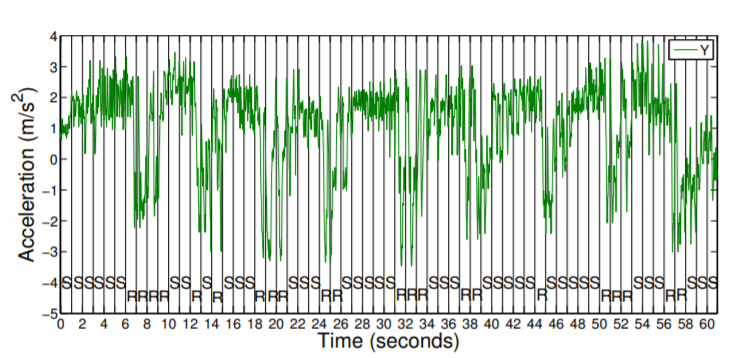
\includegraphics[width=0.75\textwidth]{Images/chapter2/relatedWork2.PNG}
   \caption{Braking events with generated class labels}
   \label{fig:graph}
    \end{figure}
    Ce  travail a été fait à Mumbai, L'algorithme identifie correctement 18 des 20 événements de bosse, Aucun tronçon de route lisse n'est identifié à tort comme une bosse. Ainsi, ils obtiennent un taux de faux négatifs de 10\% pour la détection des bosses et un taux de faux négatifs de 21,6\% et un taux de faux positifs de 2,7\% pour la détection de freinage.

  \subsection{Real time pothole detection using Android smartphones with accelerometer}
  Mednis et al., ont proposé un système de détection des nids-de-poule en temps réel basés sur des données d'accéléromètre pour le déploiement sur des appareils avec des ressources matérielles / logicielles limitées et leur évaluation sur des données du monde réel acquises à l'aide de différents téléphones intelligents basés sur Androïd OS. \newline
  ils ont utilisé un dispositif de collier LynxNet modifié \cite{PDFLynxNetWild} sur un route avec divers nids-de-poule pour la collecte des données des capteurs de l'accéléromètre.\newline 
  Après l'acquisition du premier data set de test, une recherche de fonctionnalités liées aux événements potentiels a été effectuée:\newline
  Le premier et le plus simple algorithme de détection d'événements ZTHRESH ont été testés sur l'ensemble de données acquis. Il est similaire à l'algorithme z-peak utilisé dans les systèmes Pothole Patrol \cite{PotholePatrolProceedings},Nericell\cite{mohanNericellUsingMobile2008}, et limite l'amplitude de l'accélération sur l'axe Z. Les caractéristiques qui classifient les mesures sont les valeurs dépassant des seuils spécifiques qui identifient le type des nids-de-pouls. \newline
  Pour la réorientation virtuelle, ils ont utilisé une approche plus simple: un placement contrôlé de l'accéléromètre, éliminant le traitement supplémentaire (Figure 2.3).\newline
  \begin{figure}[h!]
    \center
    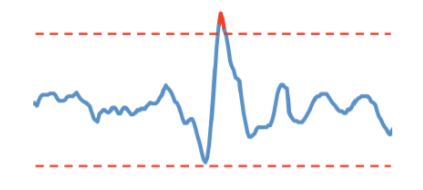
\includegraphics[width=0.75\textwidth]{Images/chapter2/relatedWork3.PNG}
   \caption{Pothole detection algorithm Z-THRESH. Events are represented by
   measurements with values exceeding specified threshold levels}
   \label{fig:graph}
    \end{figure}
    Ensuite, un algorithme légèrement plus avancé était le Z-DIFF (Figure 2.4) testé sur l'ensemble de données acquis. Contrairement à Z-THRESH, une recherche de deux mesures consécutives avec une différence entre les valeurs au-dessus du niveau de seuil spécifique a été effectuée. Ainsi, l'algorithme a détecté des changements rapides dans les données d'accélération verticale. L'algorithme nécessite la détermination de la position de l'axe Z de manière similaire à l'approche précédente. \newline
    \begin{figure}[h!]
      \center
      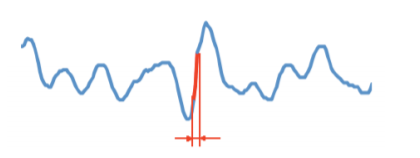
\includegraphics[width=0.75\textwidth]{Images/chapter2/relatedWork4.PNG}
     \caption{Pothole detection algorithm Z-DIFF. Events are represented by
     consecutive measurements with difference value above specific threshold level.}
     \label{fig:graph}
      \end{figure}
      les auteurs ont décidé de mettre en œuvre certaines des techniques utilisées pour le post-traitement. Une technique prometteuse pour la mise en œuvre sur un appareil à ressources limitées utilisait un écart type de l'accélération de l'axe vertical. Il a été implémenté dans l'algorithme STDEV (Z) (Figure 2.5) \newline

   \begin{figure}[h!]
      \center
      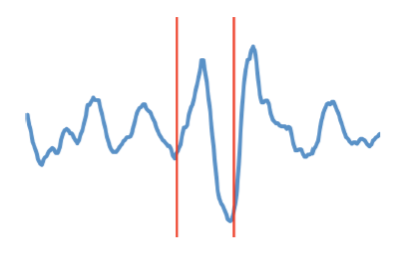
\includegraphics[width=0.75\textwidth]{Images/chapter2/relatedWork5.PNG}
     \caption{Pothole detection algorithm STDEV(Z). Events are represented by
     measurements with standard deviation value above specific threshold level.}
     \label{fig:graph}
      \end{figure}

      En utilisant des outils d'analyse visuelle de données et en recherchant des modèles de données spécifiques, les auteurs ont constaté qu'il existait certains événements caractérisés par un tuple de mesure spécifique. Toutes les données à trois axes de ce tuple avaient des valeurs proches de 0g. ils ont donc nommé cet algorithme G-ZERO (Figure 2.6).\newline


   \begin{figure}[h!]
      \center
      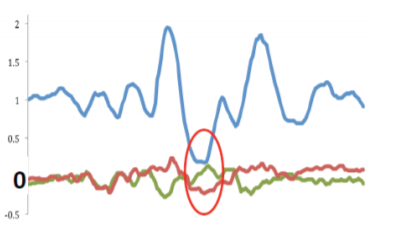
\includegraphics[width=0.75\textwidth]{Images/chapter2/relatedWork6.PNG}
     \caption{Pothole detection algorithm G-ZERO. Events are represented by tuple
     of measurements with all three axis values below specific threshold level.}
     \label{fig:graph}
      \end{figure}

      
les algorithmes ont détecté des irrégularités sur la route principale pour 100\% des grands nids-de-poule et 83 à 90\% des grappes de nids-de-poule; Selon l'algorithme, 78 à 89\% de la vérité terrain pour les petits nids-de-poule ont été détectés. Il est à noter que 9 d'entre eux (50\%) ont été détectés par les 4 algorithmes pour chacune des 10 sessions d'essai sur route
Et en gros, les tests d'évaluation ont abouti à une configuration optimale pour chaque algorithme sélectionné et l'analyse des performances dans le contexte de différentes classes d'irrégularité routière montre des taux de vrais positifs pouvant atteindre 90\%.
